%! TeX program = lualatex
\documentclass{beamer}
\usetheme{metropolis}

\setbeamerfont{page number in head/foot}{size=\tiny}
\setbeamercolor{footline}{fg=gray!70}

% Footline highlight
\colorlet{footlineHlColor}{black!60}
\newcommand{\footlineHl}[1]{
  \textbf{\textcolor{footlineHlColor}{#1}}
}

\newif\ifisdraft
\isdrafttrue
\newcommand{\todo}[1]{
  \ifisdraft {
    \Large
    $\color{black}\star$\color{red}~\textit{#1}\color{black}~$\star$
  } \fi
}

\definecolor{powderColor}{rgb}{0.878,0.859,0.811}
\definecolor{metalColor}{rgb}{0.420,0.408,0.384}
\newcommand{\legendpowderbulk}{%
  \begin{tabular}{rlrl}
     ({\color{powderColor} \rule[-1.5 pt]{8 pt}{8 pt}}) & Powder & ({\color{metalColor} \rule[-1.5 pt]{8 pt}{8 pt}})  & Bulk
  \end{tabular}
}
\newcommand{\wireframeTriangle}{%
    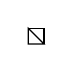
\begin{tikzpicture}[scale=0.2] % adjust scale as needed
      % Bottom triangle
      \draw[]
        (0,0) coordinate (A)
        -- (0,1) coordinate (B)
        -- (1,0) coordinate (C)
        -- cycle;
      % Upper triangle
      \draw[]
        (0,1) coordinate (D)
        -- (1,1) coordinate (E)
        -- (1,0) coordinate (F);
    \end{tikzpicture}
}

\defbeamertemplate*{title page}{customized}[1][]
{
  \usebeamerfont{title}\inserttitle\par
  \usebeamerfont{subtitle}\usebeamercolor[fg]{subtitle}\insertsubtitle\par
  \bigskip
  \usebeamerfont{author}\insertauthor\par
  \usebeamerfont{institute}\insertinstitute\par
  \usebeamerfont{date}\insertdate\par
  \usebeamercolor[fg]{titlegraphic}\inserttitlegraphic
}
\makeatletter
  \setbeamertemplate{frametitle}{%
    \begin{beamercolorbox}[%
      wd=\paperwidth,%
      sep=0pt,%
      leftskip=\metropolis@frametitle@padding,%
      rightskip=\metropolis@frametitle@padding,%
      ]{frametitle}%
      \metropolis@frametitlestrut@start%
      \insertframetitle%
      \ifx\insertframesubtitle\@empty%
      \else%
        \hfill%
        {\usebeamerfont{framesubtitle}\usebeamercolor[fg]{framesubtitle}\insertframesubtitle}%
      \fi%
      \nolinebreak%
      \metropolis@frametitlestrut@end%
    \end{beamercolorbox}%
  }
\makeatother

\usepackage{caption}
\captionsetup{font=scriptsize,labelfont=scriptsize}
\usepackage{subcaption}
\usepackage{siunitx}
\sisetup{
  range-phrase = --,
  range-units = single,
}
\usepackage{multirow}
\usepackage{booktabs}

\usepackage{cleveref}

\usepackage{natbib}

\usepackage{multimedia}

\usepackage{pifont}

% CASTEL PACKAGES
\usepackage{import}
\usepackage{xifthen}
\usepackage{transparent}
% END CASTEL PACKAGES
\newcommand{\castelincfig}[2][1.0]{%
  \def\svgwidth{#1\columnwidth} \import{./figures/}{#2.pdf_tex}
}

% Math commands
\newcommand{\dependson}[1]{
  {\scriptstyle(#1)}
}

\usepackage{calc}
\usepackage{tikz}
\usetikzlibrary{calc,positioning}
\tikzset{
  annotate box/.style={
    fill=white,
    fill opacity=.4,
    text opacity=1,
    rounded corners=2pt,
    inner xsep=4pt,
    inner ysep=3pt,
    draw=black,
    line width=.4pt,
  },
}
\DeclareRobustCommand{\labelbox}[2][]{%
  % Inline TikZ node; safe in text, math, tabular, makebox, etc.
  \tikz[baseline=(X.base)]\node[annotate box,#1] (X) {#2};%
}
\newcommand{\playthumb}[2][]{%
  \begin{tikzpicture}
    % Thumbnail image
    \node[inner sep=0] (img) {\includegraphics[#1]{#2}};
    % Dark circle
    \draw[fill=black!60, draw=white, line width=0.8pt]
      (img.center) circle[radius=0.6cm];
    % Triangle
    \draw[fill=white, draw=none, rounded corners=1.5pt]
      ([xshift=0.34cm]img.center) --
      ([xshift=-0.19cm,yshift=0.3cm]img.center) --
      ([xshift=-0.19cm,yshift=-0.3cm]img.center) -- cycle;
  \end{tikzpicture}%
}

\title{Computational strategies for time-accurate simulation of part-scale LPBF}
\subtitle{Time scale disparity in moving heat source problems}
\author{Mehdi Slimani}
\date{January 23, 2026}

\graphicspath{{figures/}}


\begin{document}

  \maketitle

  \setbeamertemplate{frame footer}{Computational strategies for time-accurate simulation of part-scale \footlineHl{LPBF}}

  \begin{frame}
    \frametitle{{LPBF}}
    \framesubtitle{MAM technology}
    Also known as PBF-LB/M (ISO nomenclature), one of the
    main Metal Additive Manufacturing (MAM) technologies

    \begin{figure}
      \begin{subfigure}[t]{0.32\textwidth}
        \centering
        \includegraphics[width=\linewidth]{waam.jpg}
        \textbf{Wire Arc Additive Manufacturing
        \raisebox{5pt}{(}\includegraphics[height=16pt]{waam-comic-effect.png}\raisebox{5pt}{)}}
      \end{subfigure}%
      \hfill
      \begin{subfigure}[t]{0.32\textwidth}
        \centering
        \includegraphics[width=\linewidth]{ded.jpg}
        \textbf{Directed Energy Deposition (DED)}
      \end{subfigure}%
      \hfill
      \begin{subfigure}[t]{0.32\textwidth}
        \centering
        \includegraphics[width=\linewidth]{lpbf.png}
        \textbf{Laser Powder Bed Fusion (LPBF)}
      \end{subfigure}
    \end{figure}
  \end{frame}

  \begin{frame}
    \frametitle{LPBF}
    \framesubtitle{How does it work?}
    \todo{Add schematic of LPBF process here.}
  \end{frame}

  \begin{frame}
    \frametitle{{LPBF}}
    \framesubtitle{Fast, small, precise}

    \begin{table}
      \centering
      \begin{tabular}{l
        S
        S
        S }
        \toprule
        & {Radius $R$} 
        & {Speed $V$} 
        & {Power $P$} \\
        \midrule
        WAAM 
          & \qtyrange[]{2}{4}{\milli\meter}
          & \qtyrange[]{3}{10}{\milli\meter\per\second}
          & \qtyrange[]{5}{15}{\kilo\watt} \\
        DED 
          & \qtyrange[]{0.5}{1.5}{\milli\meter}
          & \qtyrange[]{5}{20}{\milli\meter\per\second}
          & \qtyrange[]{1}{4}{\kilo\watt} \\
        LPBF 
          & \qtyrange[]{25}{100}{\micro\meter}
          & \qtyrange[]{400}{1400}{\milli\meter\per\second}
          & \qtyrange[]{0.2}{1}{\kilo\watt} \\
        \bottomrule
      \end{tabular}
      \caption{Characteristic heat source parameters for the main MAM technologies.}
    \end{table}

    \vspace{-3mm}
    % LPBF offers a finer resolution and smoother surface finish,
    % but it is limited to smaller parts.
    \begin{figure}
      \centering
      \begin{subfigure}[t]{0.48\textwidth}
        \centering
        \includegraphics[width=0.9\linewidth]{waam-example.jpg}\\
        {\scriptsize WAAM: large parts (> \qty{1}{\meter}), coarse features.}
      \end{subfigure}%
      \hfill
      \begin{subfigure}[t]{0.48\textwidth}
        \centering
        \includegraphics[width=0.6\linewidth]{lpbf-fine.png}\\
        {\scriptsize LPBF: small part (< \qty{1}{\meter}), fine features.}
      \end{subfigure}
    \end{figure}

  \end{frame}

  \setbeamertemplate{frame footer}{Computational strategies for time-accurate \footlineHl{simulation} of \footlineHl{part-scale} LPBF}

  \begin{frame}
    \frametitle{LPBF}
    \framesubtitle{Extremely multiscale}
    LPBF is an \textit{extremely multiscale} application \citep{hodge2021}.\\
    Let's quantify this statement:
    \begin{itemize}
      \item The \textbf{smallest} spatial and temporal \textbf{scales} are governed by the
        \textbf{heat source}, characterized by its radius $\mathbf{R}$ and by
        the time it takes to travel one radius,
        \[
          \mathbf{T_{hs}} := \frac{R}{V}.
        \]
      \item The \textbf{largest} spatial and temporal \textbf{scales} are set
        by the \textbf{part} and the printer.
        We choose here the characteristic part length $\mathbf{L_{part}}$ and
        the net printing time $\mathbf{T_{print}}$, i.e. the cumulative
        laser-on time.
    \end{itemize}
  \end{frame}

  \begin{frame}
    \frametitle{LPBF}
    \framesubtitle{Extremely multiscale}
    \centering
    \begin{minipage}{0.59\textwidth}
      \begin{figure}[ht]
        \def\svgwidth{\columnwidth}
        \import{./figures/cube-example}{cube-scan-schematic.pdf_tex}
        \caption{Cube scan path of \textbf{side length} $L$, \textbf{layer thickness} $t$
        and \textbf{hatch spacing} $h$.}
      \end{figure}
    \end{minipage}%
    \hfill%
    \begin{minipage}{0.38\textwidth}
      Consider printing a cube of side length $L$.
      The ratio of volume scales is
      $$
      \frac{L^3}{R^3}
      $$
      Let's compute the time scale ratio.
      Assume $t~=~h~=~R$ for simplicity, so that
      $$N_{layers} = N_{hatches\\/layer} = \frac{L}{R}$$
    \end{minipage}
  \end{frame}

  \begin{frame}
    \frametitle{LPBF}
    \framesubtitle{Extremely multiscale}
    For this simple geometry, the net print time is
    \begin{gather*}
      T_{print} = N_{hatches} \cdot T_{hatch} = N_{layers} \cdot N_{hatches/layer} \cdot T_{hatch}\\
      T_{hatch} = \frac{L}{V}\\
      \implies
      T_{print} = \frac{L}{R} \cdot \frac{L}{R} \cdot \frac{L}{V} = \frac{L^2}{R^2} \cdot \frac{L}{V} = \frac{L^3}{R^2 V}
    \end{gather*}
    Therefore, the time scale disparity is
    $$
    \frac{T_{print}}{T_{hs}} = \frac{L^3}{R^2 V} \cdot \frac{V}{R} = \left(\frac{L}{R}\right)^3
    $$
  \end{frame}

  \begin{frame}
    \frametitle{Part-scale simulation}
    \framesubtitle{Why?}

    We've established that LPBF is extremely multiscale.
    In a few slides, we'll see why this is a problem for
    part-scale simulation.

    Why part-scale simulation?
    \begin{itemize}
      \item Avoid costly experimental trial-and-error
      \item Predict residual stresses and distortions
      \item Predict microstructure features
      \item Optimize process parameters
      \item Save time and costs in the design cycle
    \end{itemize}
  \end{frame}

  \begin{frame}
    \frametitle{Multiphysics \todo{Better title}}
    \begin{figure}[ht]
      \centering
      \includegraphics[height=0.8\textheight]{bayat2021.png}
      \caption{Relevant physics at melt-pool and part scales \citep{bayat2021}.}
      \label{fig:bayat2021}
    \end{figure}
  \end{frame}

  \begin{frame}
    \frametitle{Problem statement}
    \framesubtitle{Domain}
    \begin{figure}[ht]
      \def\svgwidth{\columnwidth}
      \hspace{-6mm}
      \import{./figures/lpbf_schematic}{schematic.pdf_tex}
      \caption{Schematic of the LPBF computational domain 
      $\Omega(t)$, encompassing the bulk (part and substrate) and powder bed regions,
      together with the applied heat source and convective/radiative heat losses.
    }
    \end{figure}
  \end{frame}

  \begin{frame}
    \frametitle{Problem statement}
    \framesubtitle{PDE system}
    {\small
    Define the extended temperature and liquid fraction fields
    \begin{equation*}
      T_e\dependson{\mathbf{x}, t} =
      \begin{cases}
        T\dependson{\mathbf{x}, t} & \mathbf{x} \in \overline{\Omega}(t)\\
        T_{dep} & \mathbf{x} \in \overline{\Omega}(t_{final}) \setminus \overline{\Omega}(t)
      \end{cases}
      \qquad
      f_{l,\; e}\dependson{\mathbf{x}, t} = f_l(T_e\dependson{\mathbf{x}, t})
    \end{equation*}
    where $T_{dep}$ is the deposition temperature.\\
    Find $T : \Omega(t) \times [0, T_{\text{final}}] \to \mathbb{R}$ such that
    \begin{align}
      \label{eq:original_pde}
      \rho c_p \partial_t T_e + \rho L \partial_t f_{l,\; e} - k \Delta T
      &= r\dependson{\mathbf{x}, t} &&\forall \mathbf{x} \in \Omega(t)\\
      \notag
      - k \partial_n T &= h_{conv} (T - T_{\text{env}}) + \varepsilon \sigma (T^4 - T_{\text{env}}^4) &&\forall \mathbf{x} \in \partial \Omega(t)\\
      \notag
      T\dependson{\mathbf{x}, 0} &= T_0 \qquad &&\forall \mathbf{x} \in \Omega(0)
    \end{align}
    }
      \todo{Comment on phase change treatment here}
  \end{frame}

  \begin{frame}
    \frametitle{Discretization}
      Multiply \cref{eq:original_pde}
      by $\phi \in V_T(t) = H^{1}\left(\Omega(t)\right)$;
      integrate over $\Omega\dependson{t}$;
      apply integration by parts on the diffusion term; insert BCs:
      \begin{gather*}
        \label{eq:weak_heat}
        \int_{\Omega} \phi \rho \left({c_p \partial_t T + L \partial_t f_l}\right)
        + \int_{\Omega} \nabla \phi \cdot \left(k \nabla T\right)
        \;=\; \int_{\Omega} \phi r\\
        \notag
        \forall \phi \in V_T(t) \hspace{1cm}
        + \int_{\partial \Omega} \phi \left({h_{\text{conv}} \left( T - T_{\text{env}} \right)
        + \varepsilon \sigma \left( {T}^4 - T_{\text{env}}^4 \right)}\right)
      \end{gather*}
  \end{frame}

  \begin{frame}
    \frametitle{Discretization}
    \framesubtitle{Element activation}
    \begin{figure}
      \begin{subfigure}[t]{0.30\textwidth}
        \includegraphics[width=\textwidth]{schematic_melting/0.png}
        \caption{Bare substrate below an inactive powder layer.}
        \label{fig:refModelBareSubstrate}
      \end{subfigure}\hfill%
      \begin{subfigure}[t]{0.30\textwidth}
        \includegraphics[width=\textwidth]{schematic_melting/1.png}
        \caption{A powder layer is activated during a recoating step.}
        \label{fig:powderLayer}
      \end{subfigure}\hfill%
      \begin{subfigure}[t]{0.30\textwidth}
        \includegraphics[width=\textwidth]{schematic_melting/2.png}
        \caption{After a heating step, elements whose average temperature
        surpasses $T_m$ are set to bulk.}
        \label{fig:activPhaseChange3}
      \end{subfigure}\hfill%
      \caption{Illustration of deposition and melting processes.\qquad
        \legendpowderbulk{}
      }
      \label{fig:activPhaseChange}.
    \end{figure}
    Same treatment of phase change as in \citep{kollmannsberger2018}
    \todo{Maybe remove this slide, contradicting legend on next slide?}
  \end{frame}

  \begin{frame}
    \frametitle{Discretization}
    \begin{figure}
      \movie[externalviewer]{\playthumb[width=0.8\textwidth]{thumbnail-2dlpbf_2d_lpbf_ref.png}}{../videos/2dlpbf_2d_lpbf_ref.mp4}
      \caption{Demo simulation of 2D LPBF with element activation.\\
        Wireframe elements (\;\wireframeTriangle{}) correspond to powder region.
      }
    \end{figure}
    \todo{Merge with previous slide?}
  \end{frame}

  \begin{frame}
    \frametitle{Part-scale simulation}
    \framesubtitle{Impossible}
    Previous slide: ``uniform'' mesh in part and powder region.
    Recall the volume scale ratio;
    In 3D, we would need
    \begin{equation}
      \label{eq:num_elements_uniform_mesh}
      \text{\# elements} = \mathcal{O}\left(\frac{L^3}{R^3}\right)
    \end{equation}
    to resolve the heat source throughout the print.

    In practice, no one uses uniform meshes for LPBF simulation;
    \textbf{AMR} is regarded as the \textbf{de facto standard}.
  \end{frame}

  \begin{frame}
    \frametitle{Part-scale simulation}
    \framesubtitle{Impossible}
    But what about time-steps?
    The interval of interest is $]0, T_{final}[$ with
    $$
    T_{final} = T_{print} + T_{cool}
    $$
    i.e. the net printing time plus cooling.
    The time scale disparity requires again \cref{eq:num_elements_uniform_mesh} time-steps
    \begin{gather}
      \label{eq:num_timesteps_uniform_mesh}
      \text{\# time-steps} > \frac{T_{print}}{T_{hs}} = \mathcal{O}\left(\frac{L^3}{R^3}\right)\\
    \end{gather}
    when discretizing with \textbf{uniform time-steps}.
  \end{frame}

  \begin{frame}
    \frametitle{Part-scale simulation}
    \framesubtitle{Impossible}
    Intuitively, if we don't respect the constraint
    \begin{equation}
      \label{eq:origconstraint}
      \Delta t \leq T_{hs}
    \end{equation}
    , we won't resolve the motion of the heat source.\\
    In practice, that's indeed what happens:
    if the time-step is larger than $T_{hs}$ i.e. the heat source
    travels more than $1 R$ per time-step,
    it skips over parts of the domain,
    and generates artificial temperature spikes.
    \begin{figure}
      \begin{subfigure}[t]{0.49\textwidth}
        \includegraphics[width=\textwidth]{timestep-2ths/1R.png}
        \caption{$\Delta t = 1 T_{hs}$}
        \label{fig:spots1R}
      \end{subfigure}
      \begin{subfigure}[t]{0.49\textwidth}
        \includegraphics[width=\textwidth]{timestep-2ths/2R.png}
        \caption{$\Delta t = 2 T_{hs}$}
        \label{fig:spots2R}
      \end{subfigure}
      % \caption{2D heating track example with admissible and inadmissible
      % time-step sizes according to inequality \eqref{eq:origconstraint}.}
      % \label{fig:spots}
    \end{figure}
  \end{frame}

  \begin{frame}
    \frametitle{Part-scale simulation}
    \framesubtitle{Impossible}
    So \eqref{eq:num_timesteps_uniform_mesh} is indeed a \textbf{lower bound} on the number of time-steps
    when using uniform time-stepping.

    \underline{Bad news:}
    \begin{itemize}
      \item \textbf{Uniform time-stepping} is the \textbf{de facto standard} in LPBF simulation.
      \item Some references require time-steps much smaller than $T_{hs}$
        to ensure stability and accuracy \citep{hodge2014, hodge2021, elahi2025}.
    \end{itemize}
    There are basically 4 (!) groups in the world that can run simulations in the order of $\mathcal{O}(10 \unit{\milli\meter})$:
    Pittsburgh, Northwestern, LLNL, TUM.\\
    Decimeter-scale parts are currently unfeasible.
    \todo{Expand}
  \end{frame}

  \setbeamertemplate{frame footer}{Computational strategies for \footlineHl{time-accurate} simulation part-scale LPBF}

  \begin{frame}
    \frametitle{Part-scale simulation}
    \framesubtitle{Lumped heat source}
    What do you do if you don't have a cluster or a nice GPU ?
    You \textbf{simplify the model}.

    \begin{figure}
      \centering
      \def\svgwidth{0.5\textwidth}%
      {\small
      \import{./figures/goldakProfile}{profile.pdf_tex}
      }
      \caption{Double ellipsoidal profile \citep{goldak1984}.
        $\xi$ is the welding direction.}
      \label{fig:goldak}
    \end{figure}
  \end{frame}

  \begin{frame}
    \frametitle{Part-scale simulation}
    \framesubtitle{Lumped heat source}
    \begin{figure}
      \centering
      \begin{tikzpicture}
        % include the original figure
        \node[inner sep=0] (img) {\def\svgwidth{0.5\textwidth}%
          {\small \import{./figures/goldakProfile}{profile.pdf_tex}}};

        % red "forbidden" cross over the whole image
        \draw[line width=2pt, red] ([shift={(-2mm,-2mm)}]img.south west)
                                   -- ([shift={(+2mm,+2mm)}]img.north east);
        \draw[line width=2pt, red] ([shift={(+2mm,-2mm)}]img.south east)
                                   -- ([shift={(-2mm,+2mm)}]img.north west);
      \end{tikzpicture}
    \end{figure}
    We give up on the accurate representation of the heat source
    since it is too costly to resolve.

    We use a \textbf{lumped heat source} instead.
  \end{frame}

  \begin{frame}
    \frametitle{Part-scale simulation}
    \framesubtitle{Lumped heat source}
    A time-step is chosen regardless of the heat source path.
    Elements that are intersected by the heat source path
    during the time-step are \textbf{heated uniformly}.
    \begin{figure}
      \centering
      \begin{subfigure}[t]{0.495\textwidth}
        \centering
        \def\svgwidth{\textwidth}
        \import{./figures/lumped_hs}{heated_els.pdf_tex}
        \caption{Elements heated uniformly during $[t^{n},\,t^{n+1}]$.\\
             \begin{tikzpicture}
               \draw[red, very thick, dashed] (0,0.3) -- (0.4,0.3);
             \end{tikzpicture}
             $\; \rightarrow \;$ Heat source path
           }
        \label{fig:lhs_heated_els}
      \end{subfigure}%
      \hfill%
      \begin{subfigure}[t]{0.48508\columnwidth}
        \centering
        \includegraphics[width=\textwidth]{lumped_hs/tem.png}
        \caption{Resulting temperature field.}
        \label{fig:lhs_temp_field}
      \end{subfigure}
      \caption{Lumped heat source example.}
    \end{figure}
  \end{frame}

  \begin{frame}
    \frametitle{Part-scale simulation}
    \framesubtitle{Lumped heat source}
    \begin{figure}
      \begin{subfigure}[t]{0.32\textwidth}
        \centering
        \includegraphics[width=\textwidth]{chiumenti2017-lhs/chiumenti2017multipleHatches.png}
        \caption{Multiple hatches per time-step.}
      \end{subfigure}%
      \hfill
      \begin{subfigure}[t]{0.32\textwidth}
        \centering
        \includegraphics[width=\textwidth]{chiumenti2017-lhs/chiumenti2017singleLayer.png}
        \caption{Single layer per time-step.}
      \end{subfigure}%
      \hfill
      \begin{subfigure}[t]{0.32\textwidth}
        \centering
        \includegraphics[width=\textwidth]{chiumenti2017-lhs/chiumenti2017multipleLayers.png}
        \caption{4 layers per time-step.}
      \end{subfigure}
      \caption{Lumped heat input strategies from \cite{chiumenti2017b}.}
    \end{figure}
    \begin{itemize}
      \item[+] Feasible simulations
      \item[-] Distributed heat input $\;\longrightarrow\;$ temperatures below melt $\;\longrightarrow\;$ Numerical calibration (flash heating)
      \item[-] Loss of history: no resolution of heat source motion
    \end{itemize}
  \end{frame}

  \setbeamertemplate{frame footer}{\footlineHl{Computational strategies for time-accurate simulation part-scale LPBF}}

  \begin{frame}
    \frametitle{Problematic}
    \begin{itemize}
      \item AMR is regarded as necessary for part-scale LPBF simulation
        to adress spatial scale disparity.
      \item The time scale disparity is \textbf{equally} severe,
        yet uniform-time stepping is the standard.
    \end{itemize}
    $\implies$ Largely overlooked challenge:
    reduce the number of global time-steps required
    in part-scale LPBF simulation
    while retaining time-accuracy.
  \end{frame}

  \begin{frame}
    \frametitle{Objectives of this work}
    \begin{itemize}
      \item
        Review existing methods for addressing time-stepping
        challenges in MAM.
      \item
        Explore novel methods for reducing the number of time-steps
        required in LPBF modeling.
      \item
        Validate the proposed methods on realistic
        test cases.
      \item
        Validate the underlying physical models
        and numerical methods against experimental data.
      \item
        Provide realistic speedup estimates and practical implementation guidelines
        for the proposed methods.
      \item Ensure open science and reproducibility.
    \end{itemize}
  \end{frame}

  \begin{frame}
    \frametitle{Domain decomposition}
    \framesubtitle{Basics}
    We've established that the part-scale build is driven
    by the motion of a very localized heat source.

    What if we treat differently this region aka the Heat Affected Zone (HAZ)?

    We will do so via \textbf{domain decomposition} (DD).

    Let $\Omega_1$ and $\Omega_2$ be a non-overlapping decomposition of
    the domain $\Omega = \Omega_1 \sqcup \Omega_2$ such that
    $\Omega_1$ contains the HAZ;
    we will pose different problems in $\Omega_1$ and $\Omega_2$
    and enforce \textbf{transmission conditions} at the interface
    $\Gamma = \partial \Omega_1 \cap \partial \Omega_2$
  \end{frame}

  \begin{frame}
    \frametitle{Domain decomposition}
    \framesubtitle{Basics}
  \begin{figure}
    \centering
    \def\svgwidth{1.0\columnwidth}
    \import{figures/transmission_conds/}{drawing.pdf_tex}
    \caption{Non-overlapping DD schematic for a welding problem. $\Omega_1$ and $\Omega_2$
    cover the HAZ and underlying substrate, respectively. Transmission conditions
    must be satisfied at the interface $\Gamma = \partial \Omega_1 \cap \partial \Omega_2$.
    Admissible and inadmissible transmission conditions are shown in the miniature plots,
    which represent temperature fields across $\Gamma$.
    }
    \label{fig:transmission_conditions}
  \end{figure}
  \end{frame}

  \begin{frame}
    \frametitle{Advected subdomain}
      \movie[externalviewer]{\playthumb[width=1.0\textwidth]{thumbnail-chimera.png}}{../videos/chimera.mp4}
  \end{frame}

  \begin{frame}
    \frametitle{Substepping}
      \movie[externalviewer]{\playthumb[width=1.0\textwidth]{thumbnail-basic-ss.png}}{../videos/basic-demo-ss.mp4}
  \end{frame}

  \begin{frame}
    \frametitle{Advected subdomain + substepping}
      \movie[externalviewer]{\playthumb[width=1.0\textwidth]{thumbnail-basic-css.png}}{../videos/basic-demo-css.mp4}
  \end{frame}

  % \begin{frame}
  %   \frametitle{Parallel scalings}
  %   (Support slide)
  % \end{frame}
  %
  % \begin{frame}
  %   \frametitle{Is Celentano's method source-based or enthalpy-based}
  %   (Support slide)
  %     \todo{Add discussion on Celentano's method here}
  % \end{frame}
  %
  \begin{frame}
    \frametitle{Thank you!}
    \begin{figure}
      \movie[externalviewer]{\playthumb[width=0.8\textwidth]{thumbnail-thx-elya.png}}{../videos/yelya.mp4}
      \caption{Robin substepper thanks you!}
    \end{figure}
  \end{frame}


\bibliographystyle{plainnat}
\bibliography{refs}

\end{document}
